\section{Experiments}
\label{sec:experiments}

This section evaluates the algorithm of Section~\ref{sec:solution} on real data.
All results below were produced on the real UCI Adult extract ($N=48{,}842$) and the real Tax benchmark ($N=500{,}000$).

\subsection{Experimental Goals}
\label{subsec:experimental-goals}

\begin{description}
  \item[RQ1 -- Use cases.] Do the released explanations identify the semantic change a refinement actually makes, on the query pairs the paper motivates?
  \item[RQ2 -- Scalability.] How does running time depend on $k$, $N$, $\epsilon$, $|\mathcal{P}|$, $\tau$, $\gamma$, and on the choice of algorithm?
  \item[RQ3 -- Quality.] How close is the private algorithm to non-private references, measured against three separate baselines?
\end{description}

\subsection{Experimental Setup}
\label{subsec:experimental-setup}

\subsubsection{Datasets and Query Pairs}
\label{subsubsec:datasets}

\paragraph{Adult.} The real UCI Adult extract, $48{,}842$ records.
We use two refinements, denoted Adult 6.7 (occupation broadening) and Adult 6.8 (education--hours), listed in Table~\ref{tab:query-pairs}.

\paragraph{Tax.} The real Tax benchmark used in the data-cleaning literature, $500{,}000$ records, with the marital-status refinement denoted Tax 6.6 in Table~\ref{tab:query-pairs}.

\paragraph{Not evaluated.}
IPUMS-CPS and the Stack Overflow Developer Survey are not included in this pass, and the Hospital/CQA setting is not evaluated at all: the framework has only ever been exercised on query-refinement pairs, never on a repair-semantics pair, and doing so would additionally require implementing repair semantics.
Section~\ref{sec:usecase-results} therefore substantiates the query-refinement use case only.

\begin{table}[t]
\centering
\small
\caption{Query pairs, on the real data. Each $Q$ violates its representation constraint and each $Q'$ satisfies it.}
\label{tab:query-pairs}
\begin{tabular}{@{}llrrr@{}}
\toprule
Pair & Constraint & $|Q|$ & $|Q'|$ & share in $Q\rightarrow Q'$ \\
\midrule
Adult 6.7  & $\ge25\%$ female   & 5{,}447  & 37{,}155  & $4.7\%\rightarrow26.9\%$ \\
Adult 6.8  & $\ge25\%$ female   & 3{,}055  & 2{,}453   & $19.5\%\rightarrow30.6\%$ \\
Tax 6.6    & $\ge30\%$ HasChild & 145{,}576 & 291{,}659 & $3.5\%\rightarrow50.1\%$ \\
\bottomrule
\end{tabular}
\end{table}

The Adult 6.8 figures reproduce the numbers quoted in Section~\ref{sec:introduction} ($19.5\%\rightarrow30.6\%$) exactly, on the real data.

\subsubsection{Parameters}
\label{subsubsec:parameters}

Unless stated otherwise $k=5$, $\lambda=0.5$, $\epsilon=1$, and the budget is split equally, $(\epsilon_P,\epsilon_S,\epsilon_H)=(\epsilon/3,\epsilon/3,\epsilon/3)$; $\tau$ and $\gamma$ follow Eqs.~\eqref{eq:tau-rule} and~\eqref{eq:gamma-rule}, giving $\tau=15$ and $\gamma\approx150$ on both datasets.
Equal shares is not an arbitrary default: sweeping the split over the three query pairs found no allocation that dominates it.
Equal shares gave the lowest released-histogram error on all three, and the best selection quality on the hardest of them.
Starving the view stage is the one clearly bad choice, since the explanation stage can only choose among the views that survive it: at $(0.10,0.55,0.35)$ the approximation ratio on Adult education-hours falls from $0.89$ to $0.57$.
Moving budget the other way buys a few points of selection quality on that pair alone and costs histogram accuracy on all three.
\alon{TODO: all numbers below were produced with $\tau=35$ and $\gamma=\lceil0.005N\rceil$ ($244$ for Adult, $2{,}500$ for Tax). They must be re-run under Eqs.~(\ref{eq:tau-rule}) and~(\ref{eq:gamma-rule}), \added{and now also under Eq.~(\ref{eq:gammaR-rule}), $\gamma_R=N/100$ in place of $\gamma_R=N$, with the view-stage sensitivity $\Delta=4/|D|$ of Proposition~\ref{prop:usefulness-sensitivity} in place of $7/(4|D|)$}. A first look on Adult education-hours, scored against a fixed yardstick so the comparison does not move with $\gamma$, put the new setting ahead of the old one, so the rerun is expected to improve rather than weaken the results.}
\alon{TODO (experiment to add): measure the view stage in isolation. For each query pair and each $\epsilon_P$, report the overlap between the privately retained $\tau$ views and the exact top-$\tau$ by $\Use$, and the lowest $\Use$ actually retained against the true $\tau$-th best. A first look at Adult education-hours suggests the overlap is low at the budgets used here and rises sharply with $\epsilon_P$, which would explain why the view stage is the one that must not be starved (Section~\ref{subsubsec:parameters}) and would give Section~\ref{subsec:two-stages} the empirical counterpart to the utility guarantee it lacks.}

Reported quantities average $40$ trials; this count is not incidental, as the between-trial standard deviation of set score is frequently comparable to its mean, and smaller counts cannot separate configurations reliably.

\subsection{Compared Methods}
\label{subsec:compared-methods}

We compare the algorithm of Section~\ref{sec:solution} against three baselines.

\begin{description}
  \item[B1 --- $\epsilon\rightarrow\infty$.] The identical algorithm, run with a privacy budget large enough that every mechanism is numerically deterministic. Isolates the cost of privacy noise alone, holding the architecture fixed.
  \item[B2 --- exhaustive optimum, non-private.] Enumerates \emph{all} size-$k$ subsets of the candidate explanations, scores each with the set-level objective of Definition~\ref{def:setobj}, and returns the maximiser.
  \item[B3 --- greedy, non-private.] Takes the top-$\tau$ views by $Usefulness$ with no privacy mechanism, then performs $k$ rounds selecting the best remaining histogram with no privacy mechanism.
\end{description}

B2 is exponential in $k$: with $\tau=35$ views and $10$ attributes the candidate space holds $350$ explanations and $\binom{350}{5}\approx5\times10^{11}$ subsets, which is not enumerable.
It is nevertheless computed \emph{exactly}, by restricting the search to the union over attributes of the top-$k$ candidates of each attribute group.
That restriction is lossless: if an optimal set contained a candidate outside the top-$k$ of its own group, some higher-scoring member of that group would be unused, and swapping it in cannot decrease $F_\lambda$, which is non-decreasing in the score of every member.
The pool is therefore $k\,|Attrs|=50$ candidates and $\binom{50}{5}\approx2.1\times10^{6}$ subsets, and B2 is the true optimum of the $\tau$-filtered space rather than an approximation to it.

\paragraph{Scoring.}
All four methods are scored on their output \emph{set} under one common yardstick: the paper's own objective, Definition~\ref{def:hd} with $\gamma_{\text{eval}}=0$, combined with the set-level utility of Definition~\ref{def:setobj}.
This is deliberate. Smoothing is a mechanism-internal device, and allowing it to define the metric as well would make the comparison circular; scoring at $\gamma_{\text{eval}}=0$ means the algorithm is judged by the standard of the unmodified paper even though it selects under smoothing.

\subsection{Use Case Results}
\label{sec:usecase-results}

\begin{figure}[t]
\centering
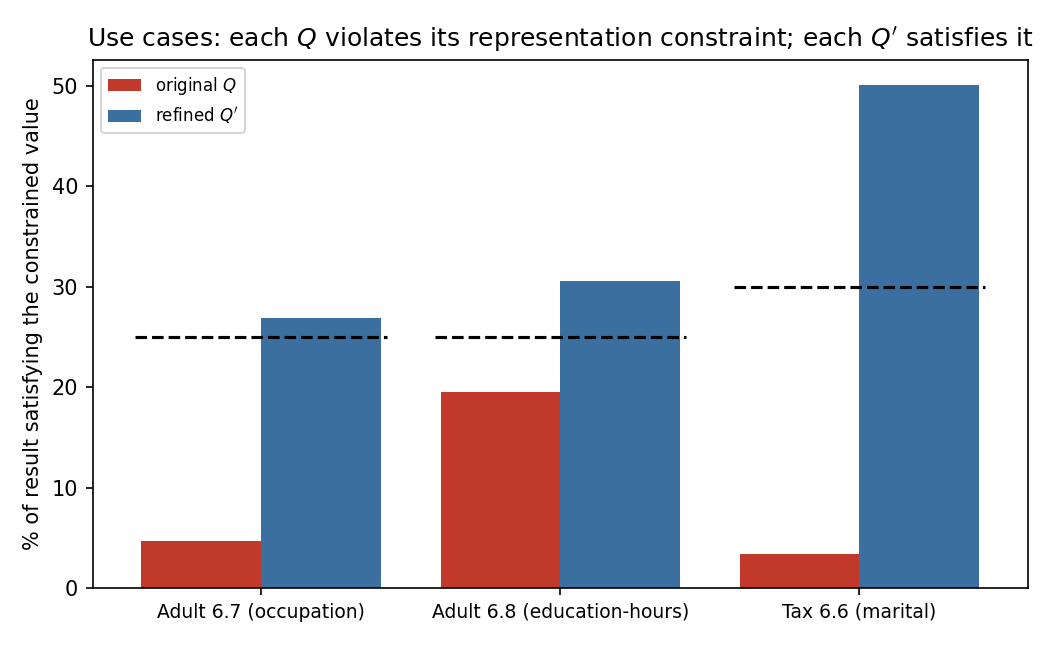
\includegraphics[width=\linewidth]{figures/U1_constraint_premise.png}
\caption{Each original query violates its representation constraint (dashed line) and each refined query satisfies it, on the real data.}
\label{fig:premise}
\end{figure}

Figure~\ref{fig:premise} establishes the premise: on real data all three refinements do what the motivating examples claim.
Figures~\ref{fig:rel-tax}--\ref{fig:rel-adult-edu} show the differentially private explanations the algorithm releases for each pair at $\epsilon=1$, $k=5$.

\begin{figure}[t]
\centering
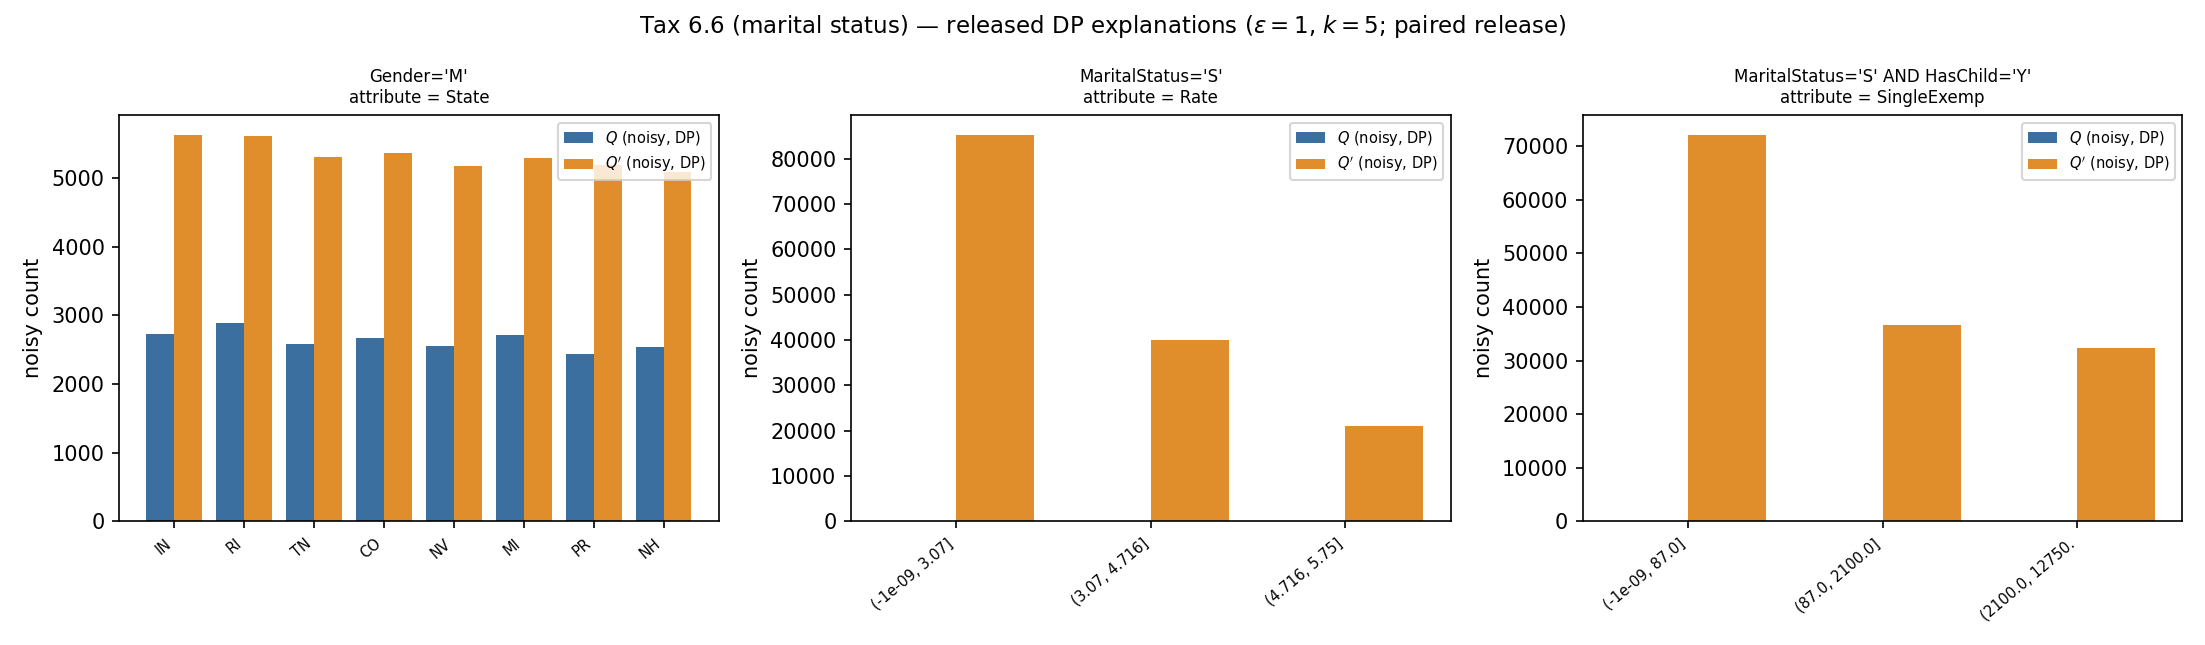
\includegraphics[width=\linewidth]{figures/U2_released_tax_marital.png}
\caption{Tax 6.6 --- released differentially private explanations.}
\label{fig:rel-tax}
\end{figure}

For Tax the refinement removes the predicate $\texttt{MaritalStatus}=\texttt{'M'}$.
The algorithm recovers exactly that subgroup: three of the five released explanations are conditioned on $\texttt{MaritalStatus}=\texttt{'S'}$, the population the refinement mechanically introduces, with a shift of $-85{,}178$ tuples concentrated in the lowest \texttt{Rate} bucket.
The framework is never given the query predicates.

\begin{figure}[t]
\centering
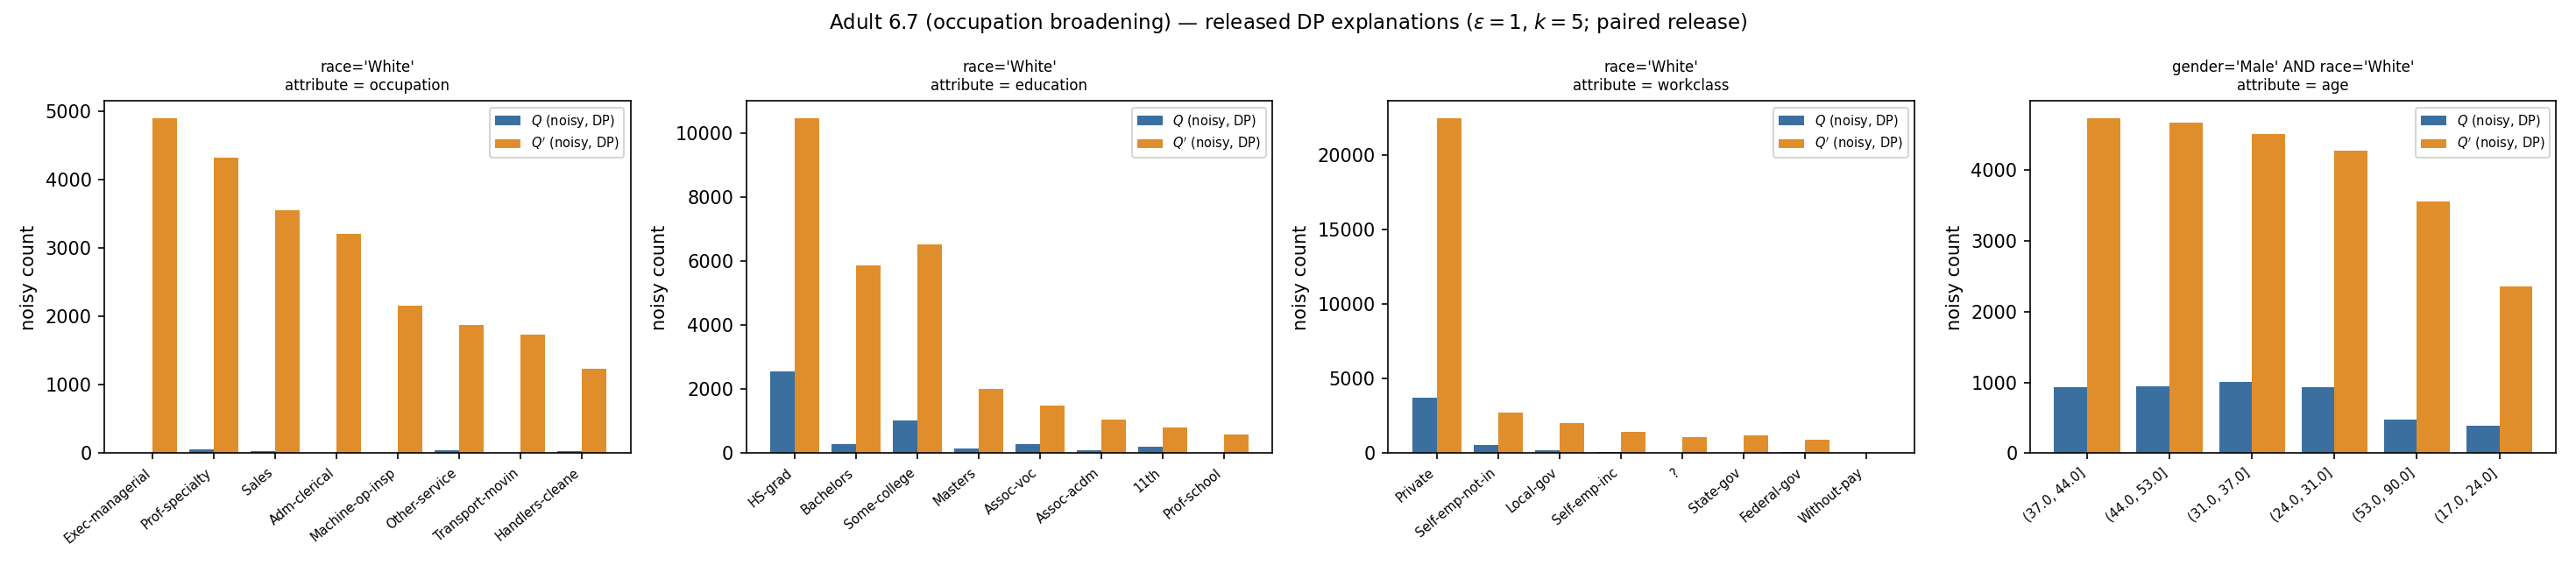
\includegraphics[width=\linewidth]{figures/U2_released_adult_occupation.png}
\caption{Adult 6.7 --- released differentially private explanations.}
\label{fig:rel-adult-occ}
\end{figure}

\begin{figure}[t]
\centering
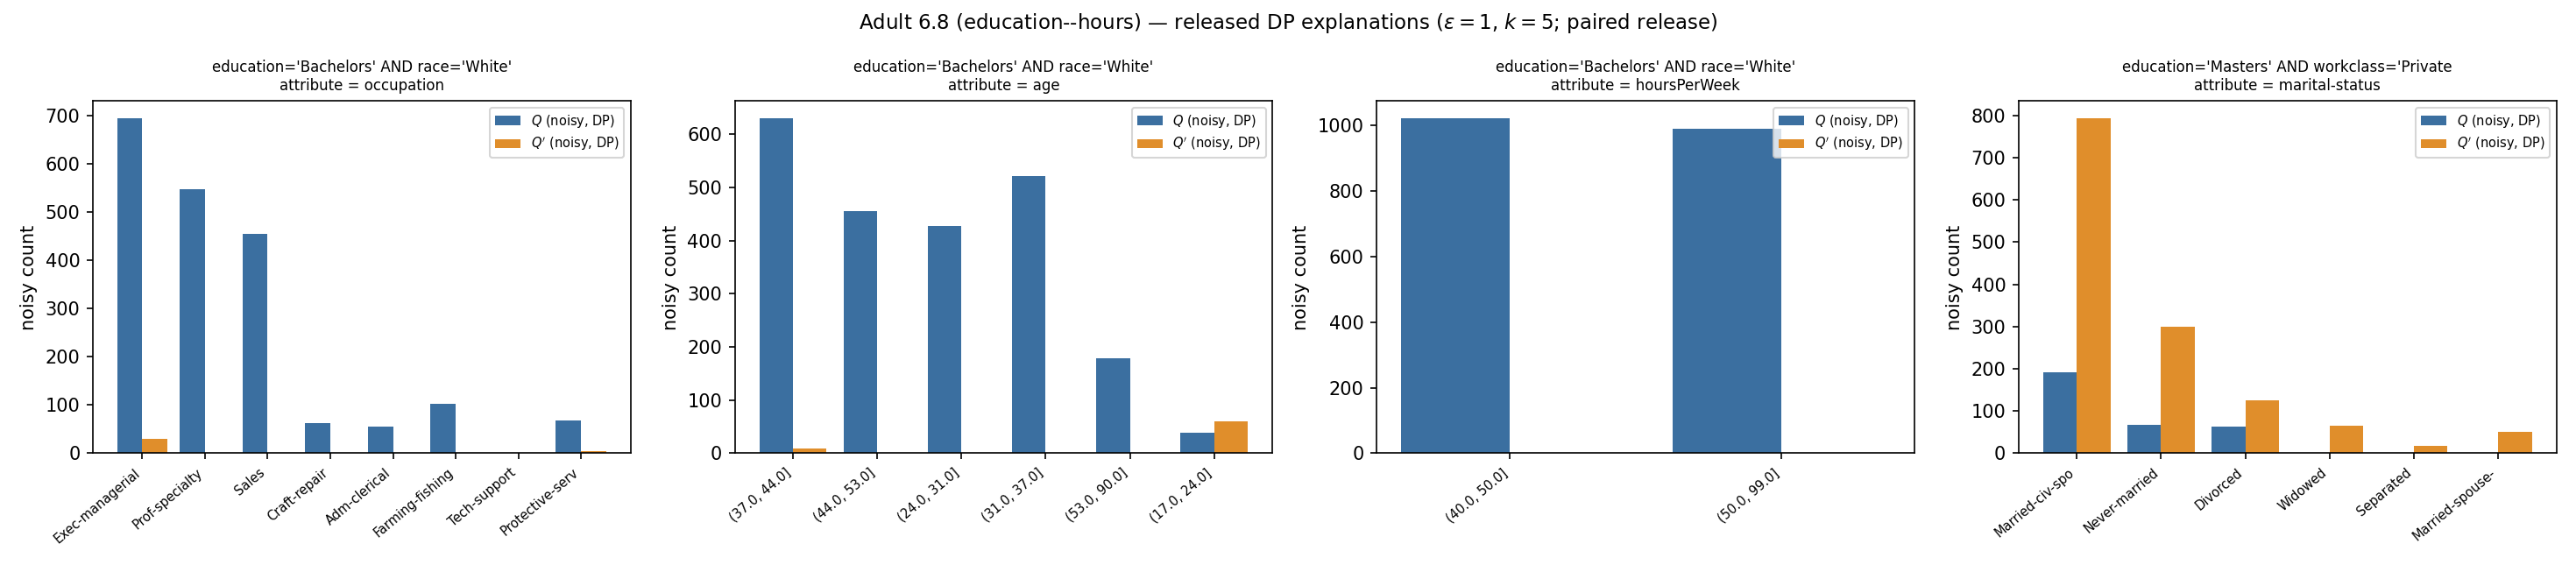
\includegraphics[width=\linewidth]{figures/U2_released_adult_education_hours.png}
\caption{Adult 6.8 --- released differentially private explanations.}
\label{fig:rel-adult-edu}
\end{figure}

For Adult 6.7 the released explanations are dominated by shifts \emph{within} $\texttt{race}=\texttt{'White'}$ across \texttt{occupation}, \texttt{education} and \texttt{workclass}, showing that broadening a narrow occupational query changes the occupational and educational composition of the result rather than merely enlarging it.
For Adult 6.8 the explanations localise on $\texttt{education}=\texttt{'Bachelors'}$ subgroups, which is the population the refinement removes when it restricts education to \texttt{Masters}.

These are the un-cherry-picked outputs of a single run at the default parameters.

\subsection{Scalability}
\label{subsec:scalability}

\begin{figure*}[t]
\centering
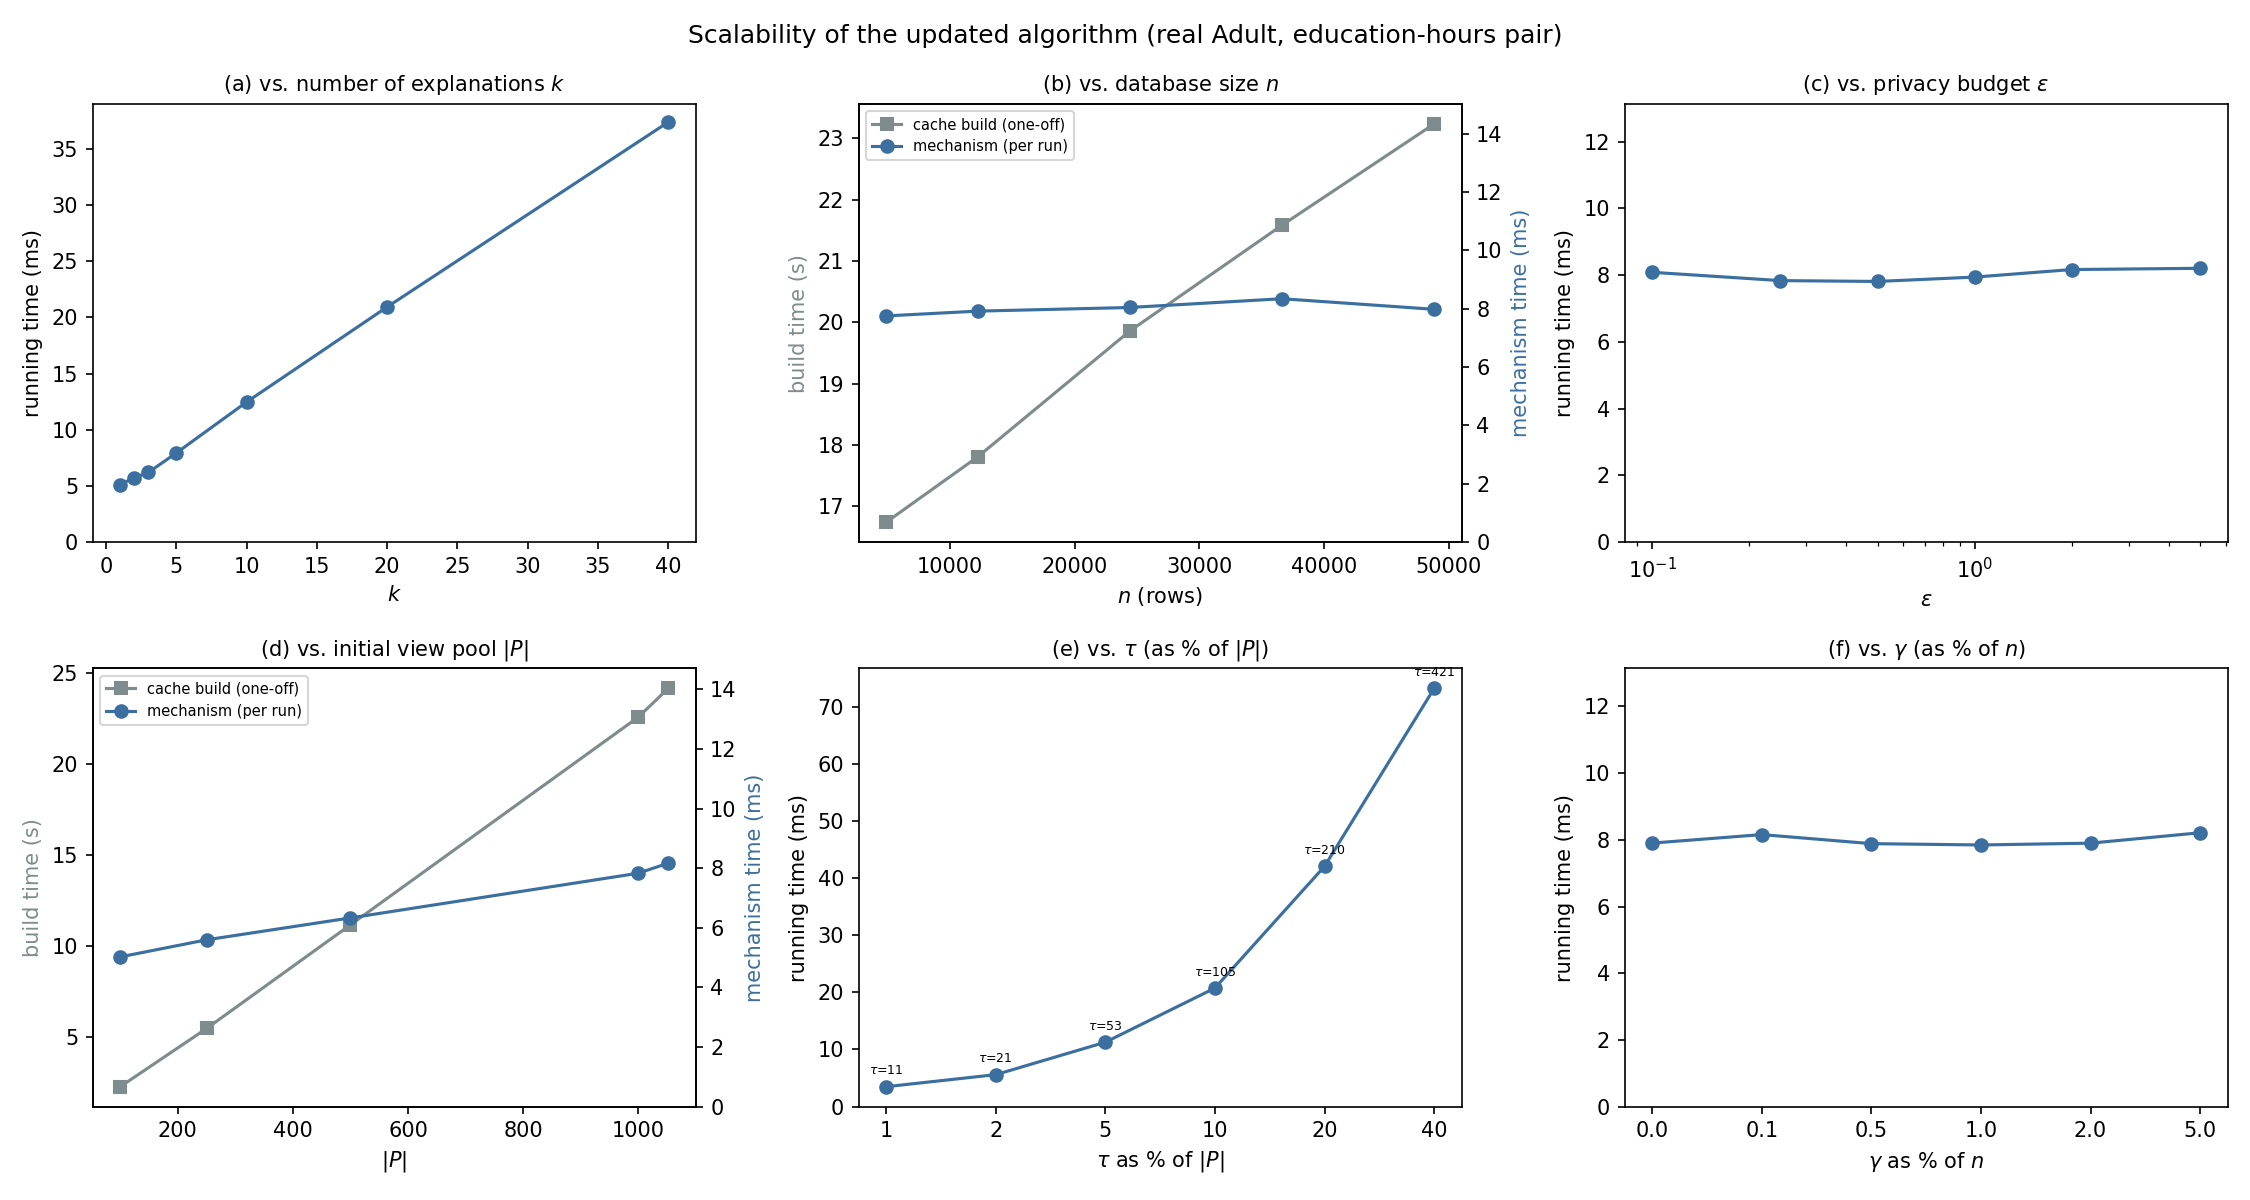
\includegraphics[width=\linewidth]{figures/S1_scalability_grid.png}
\caption{Running time of the algorithm. Panels (b) and (d) separate the one-off cache build, which carries the $O(N)$ and $O(|\mathcal{P}|)$ work, from the per-invocation mechanism cost.}
\label{fig:scalability}
\end{figure*}

Figure~\ref{fig:scalability} reports the six sweeps.

\paragraph{$k$, $\tau$, $|\mathcal{P}|$.}
Running time is linear in $k$ ($4.6$\,ms at $k=1$ to $36.3$\,ms at $k=40$) and in $\tau$, matching the $O(k\tau m b)$ term of Section~\ref{subsec:complexity-analysis}.
Expressed as a fraction of $|\mathcal{P}|$, moving $\tau$ from $5\%$ to $10\%$ doubles per-round cost ($11.1$\,ms to $19.9$\,ms) and from $5\%$ to $40\%$ multiplies it sevenfold.

\paragraph{$N$ and $|\mathcal{P}|$.}
The per-invocation cost is essentially flat in $N$ ($7.7$--$8.3$\,ms across a tenfold range), because the $O(N)$ work is confined to the one-off preprocessing, which grows from $16.7$\,s to $23.2$\,s over the same range.
Panels (b) and (d) plot both; presenting only the per-run curve on an autoscaled axis would turn a sub-millisecond spread into an apparent trend.

\paragraph{$\epsilon$ and $\gamma$.}
Running time is invariant to both ($7.8$--$8.2$\,ms across $\epsilon\in[0.1,5]$, and $7.9$--$8.3$\,ms across $\gamma$ from $0\%$ to $5\%$ of $N$).
For $\epsilon$ this is the expected result and confirms no budget-dependent overhead.
For $\gamma$ it is a consequence of the caching described in Section~\ref{subsec:complexity-analysis}: $\gamma$ enters only the denominator, so changing it costs nothing.
This is what makes re-scoring at a different $\gamma$ free in running time as well as in privacy.

\subsubsection{Running Time by Algorithm}
\label{subsec:runtime-algorithm}

\begin{figure}[t]
\centering
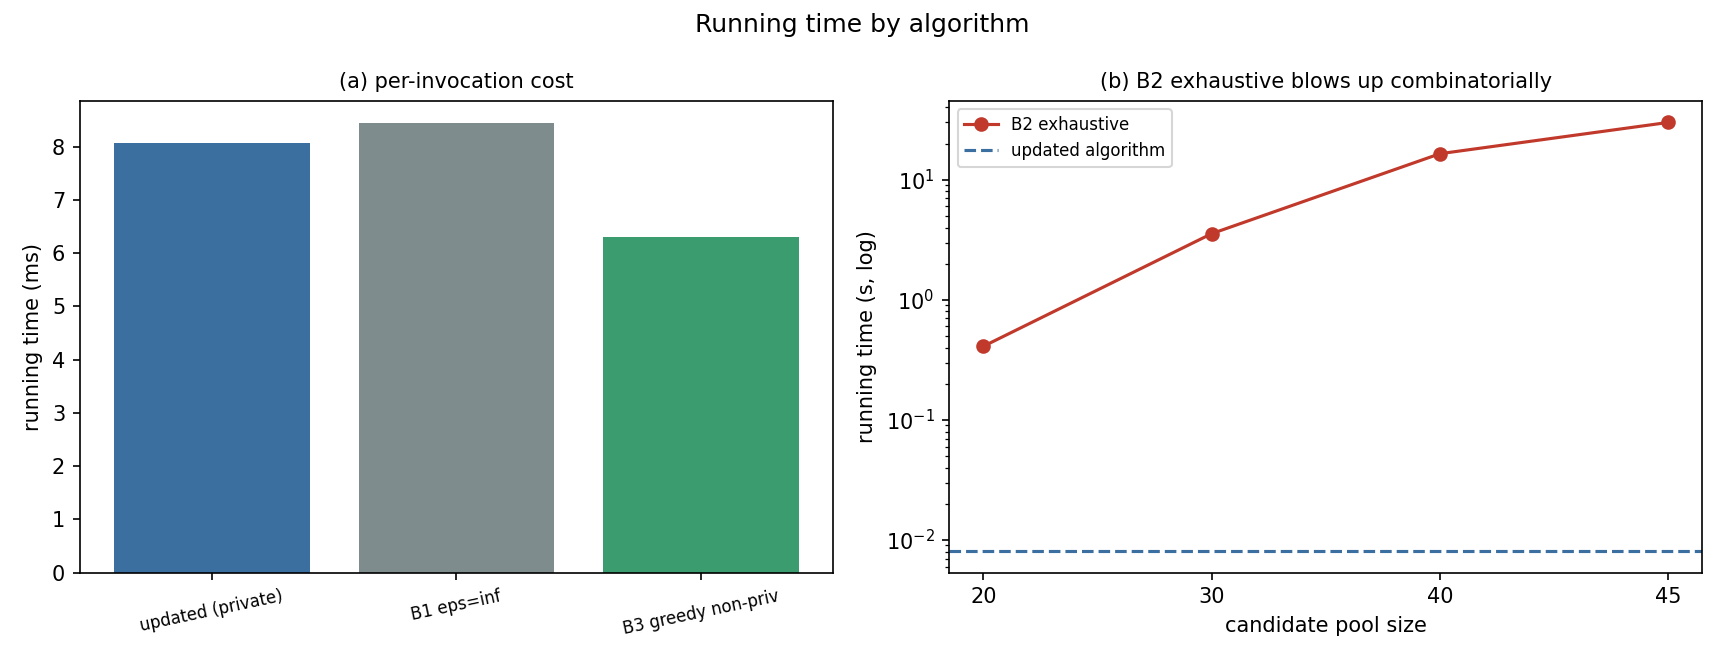
\includegraphics[width=\linewidth]{figures/S2_runtime_by_algorithm.png}
\caption{Per-invocation cost of each method, and the combinatorial blow-up of the exhaustive baseline B2.}
\label{fig:runtime-algorithm}
\end{figure}

The private algorithm ($8.1$\,ms), B1 ($8.4$\,ms) and B3 ($6.3$\,ms) are all within a small constant of one another: privacy costs essentially nothing in running time, since the exponential mechanism replaces an $\arg\max$ over the same scores.

B2 is different in kind.
On a $20$-candidate pool it takes $0.41$\,s; at $30$, $3.6$\,s; at $40$, $16.5$\,s; at $45$, $30.0$\,s --- a $73\times$ increase for a $2.25\times$ increase in pool size, tracking $\binom{|C|}{5}$.
On the lossless $50$-candidate pool it takes $57$\,s, versus $8$\,ms for the private algorithm.
Enumerating the unrestricted $350$-candidate space would take on the order of months, which is why the losslessness argument above is needed rather than optional, and why the selection is run greedily: by Proposition~\ref{prop:greedy-exact} that costs nothing in quality.

\subsection{Quality}
\label{subsec:quality}

\begin{figure*}[t]
\centering
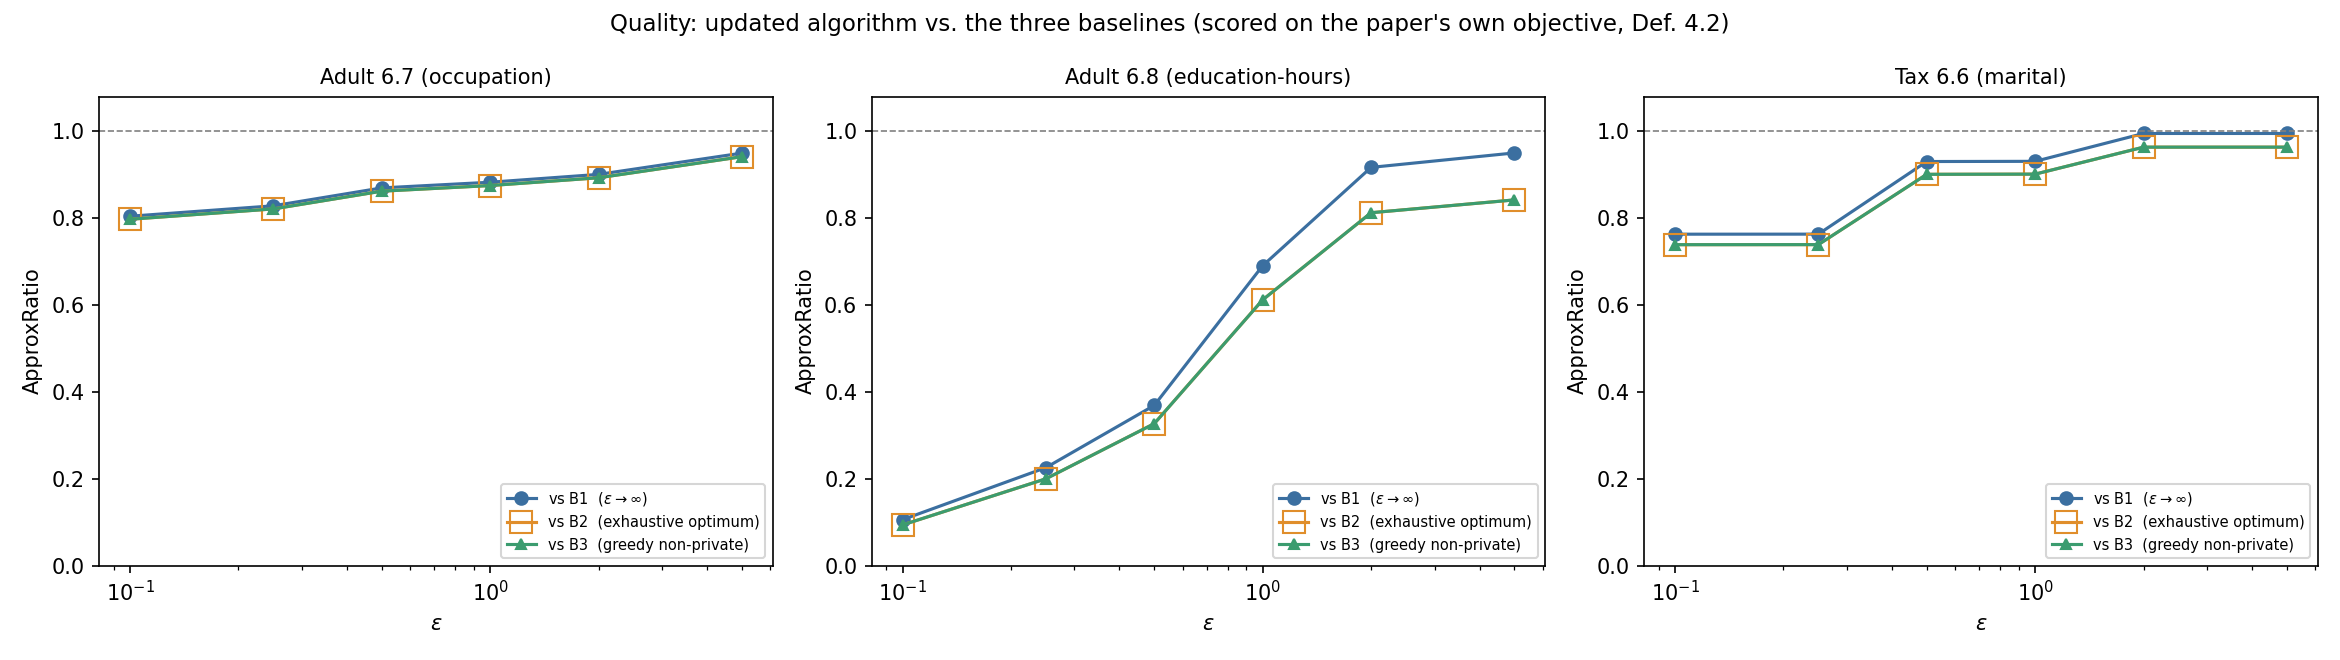
\includegraphics[width=\linewidth]{figures/Q1_approxratio_vs_baselines.png}
\caption{ApproxRatio of the algorithm against each baseline, scored on the paper's own objective ($\gamma_{\text{eval}}=0$), $40$ trials per point.}
\label{fig:quality}
\end{figure*}

\begin{table}[t]
\centering
\small
\caption{ApproxRatio against each baseline at $\epsilon=1$ and $\epsilon=5$.}
\label{tab:quality}
\begin{tabular}{@{}lcccccc@{}}
\toprule
& \multicolumn{3}{c}{$\epsilon=1$} & \multicolumn{3}{c}{$\epsilon=5$}\\
\cmidrule(lr){2-4}\cmidrule(lr){5-7}
Pair & B1 & B2 & B3 & B1 & B2 & B3\\
\midrule
Adult 6.7 & 0.883 & 0.875 & 0.875 & 0.950 & 0.941 & 0.941\\
Adult 6.8 & 0.691 & 0.612 & 0.612 & 0.950 & 0.842 & 0.842\\
Tax 6.6   & 0.931 & 0.901 & 0.901 & 0.995 & 0.963 & 0.963\\
\bottomrule
\end{tabular}
\end{table}

At the default $\epsilon=1$ the algorithm attains $0.88$--$0.93$ of the $\epsilon\rightarrow\infty$ reference on two of the three pairs and $0.88$--$0.90$ of the exhaustive optimum, rising to $0.94$--$1.00$ and $0.94$--$0.96$ respectively at $\epsilon=5$.
Adult 6.8 is the hardest pair and the only one that degrades sharply at small $\epsilon$ ($0.11$ against B1 at $\epsilon=0.1$); it is also the pair whose top candidates are most tightly bunched, so the exponential mechanism has the least separation to exploit.

Two observations are worth isolating.

First, \textbf{B2 and B3 coincide exactly on all three query pairs} (Figure~\ref{fig:absolute}): the non-private greedy procedure attains the true optimum of the $\tau$-filtered space, not merely an approximation to it.
This is what Proposition~\ref{prop:greedy-exact} predicts: on a fixed candidate set and a fixed $\gamma$ greedy returns the exact maximiser, so the two references answer the same question here.
The measurement confirms it on real instances rather than establishing it.

Second, the ratio against B2/B3 is consistently slightly below the ratio against B1.
B1 holds the architecture fixed and removes only the noise, so it isolates the cost of privacy; B2/B3 remove the noise \emph{and} search without a privacy-imposed $\tau$ budget, so the residual gap to them also includes what the mechanism gives up by having to select views privately at all.
Reporting both separates those two costs.

\begin{figure}[t]
\centering
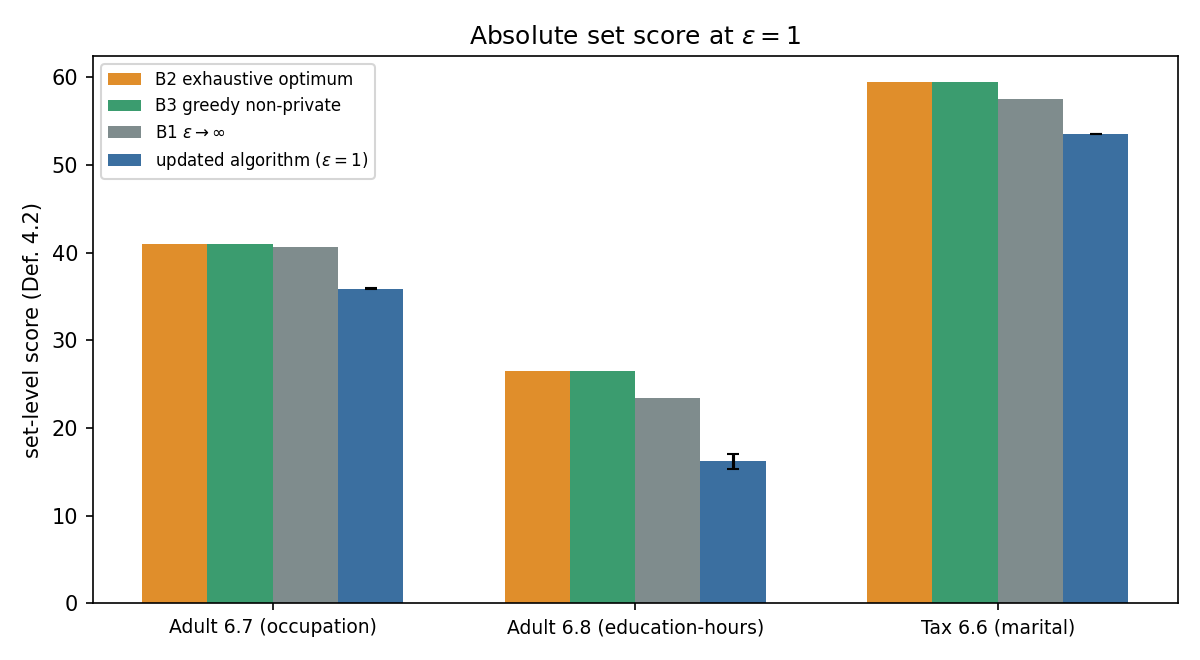
\includegraphics[width=\linewidth]{figures/Q2_absolute_scores.png}
\caption{Absolute set scores at $\epsilon=1$. B2 and B3 coincide exactly: non-private greedy attains the exhaustive optimum on every pair.}
\label{fig:absolute}
\end{figure}

\subsubsection{The $\gamma$ Trade-off}
\label{subsec:gamma-tradeoff}

Smoothing is not free, and the cost is worth stating precisely.
$\gamma$ competes against the size of individual histogram \emph{bins}, and the bin-count distribution relative to $|D|$ differs sharply between datasets: the median non-empty bin holds $20$ tuples on Adult but $3{,}897$ on Tax, a factor of $200$ despite only a factor of $10$ in $N$.
Consequently the same "fraction of $N$" rule lands in very different regimes.
At $\gamma=0.5\%$ of $N$, $\gamma$ exceeds the bin count for $84\%$ of Adult bins but only $30\%$ of Tax bins; at $5\%$ of $N$ it exceeds $98\%$ and $94\%$ respectively, at which point the median ratio $m_v/(m_v+\gamma)$ falls to $0.008$ on Adult and $HD_\gamma$ has effectively stopped measuring \emph{relative} change at all.

The pre-registered rule of Section~\ref{subsubsec:parameters} is therefore defensible but crude, and $\gamma$ at $5\%$ of $N$ would be clearly too aggressive.
A sharper anchor follows from Proposition~\ref{prop:hd-sensitivity}: the separation available to the exponential mechanism scales as $\epsilon\,\delta u\,(1+\gamma)/2$, so the $\gamma$ actually required is governed by the \emph{margin} between the leading candidates rather than by $N$.
Measured on the three pairs, that margin is $0.027$, $0.121$ and $0.315$ respectively, implying required $\gamma$ of roughly $292$, $66$ and $25$ --- an ordering unrelated to dataset size, and inverted with respect to it.

\subsection{Summary of Findings}
\label{subsec:experiments-summary}

Running time is linear in $k$, $\tau$ and $|\mathcal{P}|$, invariant to $\epsilon$ and $\gamma$, and independent of $N$ once preprocessing is amortised; privacy adds no measurable cost relative to the non-private greedy baseline, while the exhaustive baseline is intractable beyond a few dozen candidates.
On quality the algorithm reaches $0.88$--$0.93$ of the $\epsilon\rightarrow\infty$ reference at the default budget and $0.95$--$1.00$ at $\epsilon=5$, judged by the paper's own unsmoothed objective; non-private greedy attains the exhaustive optimum exactly on all three pairs, as Proposition~\ref{prop:greedy-exact} predicts.
The use cases show that the released explanations localise the population a refinement adds or removes without being given the query predicates --- most sharply on Tax, where three of five released explanations recover exactly the subgroup the dropped predicate introduces.
The principal caveat is the choice of $\gamma$: it is what makes private selection work at these budgets, but anchoring it to a fraction of $|D|$ is a crude proxy for the quantity that actually determines it.
